\chapter{Physically Based Rendering}

In order to generate photorealistic images, renderers must find accurate solutions to the \textit{rendering equation}. This chapter explains the meaning and intuition behind the equation, and describes how it can be solved by the path-tracing algorithm.

\section{The Rendering Equation}

The rendering equation describes the ``strength'' of light at each point in space and in each direction. To formalize the notion of strength, this section begins by introducing a few concepts from the study of radiometry.

\subsection{Radiometry}

In radiometry, there is a hierarchy of quantities that measures the strength of light in different contexts. The first quantity is \textit{radiant flux}, which measures the total energy that travels through a region of space per unit time in the form of electromagnetic radiation. Radiant flux is often denoted by $\Phi$, and its unit of measure is Watts($W$). 

In almost all regions in any scene, the radiant flux is not uniformly distributed, and thus one important quantity is the density of radiant flux with respect to area. This quantity is named \textit{irradiance}, which is denoted by $E$, and measured in power per unit area ($W\cdot m^{-2}$). Intuitively, irradiance measures the amount of light received by a single point in space. For this reason, for a region of space $S$, integrating the irradiance of each point in $S$ gives the total flux through $S$:
\begin{align}
    \Phi(S) = \int_S E(p) dp 
    \label{irradiance integral}
\end{align}

For any point $p$, the irradiance $E(p)$ is not uniform across all directions, and thus it is also important to consider the density of irradiance in each direction $\omega$. This quantity, $L(p,\omega)$, is called \textit{radiance}, and its unit of measure for radiance is power per unit area per unit solid angle ($\text{W}\cdot\text{m}^{-2}\cdot \text{sr}^{-1}$). Radiance is an especially important quantity, because it is a measure of the strength of a single ray of light, identified by its direction $\omega$ and a point $p$ which it passes through. Consequently, radiance is the physical quantity that ray-tracing algorithms constantly operates in. 


In rendering, radiance often appears in the form $L_o(p,\omega)$ or $L_i(p,\omega)$, which mean radiance going out from the point $p$ or entering into it, respectively. More precisely, $L_o(p,\omega)$ represents the radiance that travels from $p$ and outwards in the direction $\omega$, and $L_i(p,\omega)$ represents the incoming radiance that travels towards to $p$ in the direction $-\omega$. The convention $L_i(p,\omega)$ might appear slightly counter-intuitive, since $\omega$ points in the opposite direction as the propagation of energy. However, the convenience of this notation will become apparent when the ray-tracing algorithm is formulated. 



\begin{figure}[H]
\centering
\tikzset{every picture/.style={line width=0.75pt}} %set default line width to 0.75pt        
\begin{tikzpicture}[x=0.75pt,y=0.75pt,yscale=-1,xscale=1]
%uncomment if require: \path (0,300); %set diagram left start at 0, and has height of 300

%Straight Lines [id:da6428603089338014] 
\draw    (70,220) -- (251,220) ;
\draw [shift={(160.5,220)}, rotate = 0] [color={rgb, 255:red, 0; green, 0; blue, 0 }  ][fill={rgb, 255:red, 0; green, 0; blue, 0 }  ][line width=0.75]      (0, 0) circle [x radius= 3.35, y radius= 3.35]   ;
%Straight Lines [id:da0998330538982608] 
\draw    (160.5,220) -- (218.58,162.41) ;
\draw [shift={(220,161)}, rotate = 495.24] [color={rgb, 255:red, 0; green, 0; blue, 0 }  ][line width=0.75]    (10.93,-3.29) .. controls (6.95,-1.4) and (3.31,-0.3) .. (0,0) .. controls (3.31,0.3) and (6.95,1.4) .. (10.93,3.29)   ;
%Straight Lines [id:da7334390340946089] 
\draw    (325,221) -- (506,221) ;
\draw [shift={(415.5,221)}, rotate = 0] [color={rgb, 255:red, 0; green, 0; blue, 0 }  ][fill={rgb, 255:red, 0; green, 0; blue, 0 }  ][line width=0.75]      (0, 0) circle [x radius= 3.35, y radius= 3.35]   ;
%Straight Lines [id:da024849495612862427] 
\draw    (480,160) -- (416.95,219.63) ;
\draw [shift={(415.5,221)}, rotate = 316.6] [color={rgb, 255:red, 0; green, 0; blue, 0 }  ][line width=0.75]    (10.93,-3.29) .. controls (6.95,-1.4) and (3.31,-0.3) .. (0,0) .. controls (3.31,0.3) and (6.95,1.4) .. (10.93,3.29)   ;
%Image [id:dp8436986937138125] 
\draw (161,245) node  {
\includegraphics[width=27pt,height=30pt]{lightbulb.png}};
%Image [id:dp5859653893638117] 
\draw (498,154) node  {
\includegraphics[width=27pt,height=30pt]{lightbulb.png}};

% Text Node
\draw (181,232) node [anchor=north west][inner sep=0.75pt]   [align=left] {$\displaystyle p$};
% Text Node
\draw (224,143) node [anchor=north west][inner sep=0.75pt]   [align=left] {$\displaystyle q$};
% Text Node
\draw (436,233) node [anchor=north west][inner sep=0.75pt]   [align=left] {$\displaystyle p$};
% Text Node
\draw (519,141) node [anchor=north west][inner sep=0.75pt]   [align=left] {$\displaystyle q$};


\end{tikzpicture}

\caption{Example: consider two points $p$, $q$, and $\omega=\frac{q-p}{|q-p|}$. On the left, the radiance sent from $p$ to $q$ is $L_o(p,\omega)$. On the right, the radiance received by $p$ from $q$ is $L_i(p,\omega)$.}
\end{figure}
Similar to equation \ref{irradiance integral}, which expresses flux as an integral of irradiance, it's also possible to obtain the incoming irradiance $E(p)$ by an integral across the incoming radiance from each direction. More precisely, the following relationship holds:
\begin{align}
    E(p) = \int_\Omega L_i(p,\omega_i)\cos\theta_id\omega_i
    \label{radiance integral}
\end{align}
Here, the support $\Omega$ is often a sphere or hemisphere of possible incoming direction, and the angle $\theta_i$ represents the angle between $\omega_i$ and the surface normal. The cosine term accounts for the fact that for incoming rays that are not perfectly perpendicular to the surface, the differential area illuminated by the ray is multiplied by a factor $\frac{1}{\cos\theta_i}$, and thus the contribution per unit area should be multiplied by $\cos\theta_i$. 
\begin{figure}[H]
    \centering
  



    \tikzset{every picture/.style={line width=0.75pt}} %set default line width to 0.75pt        

    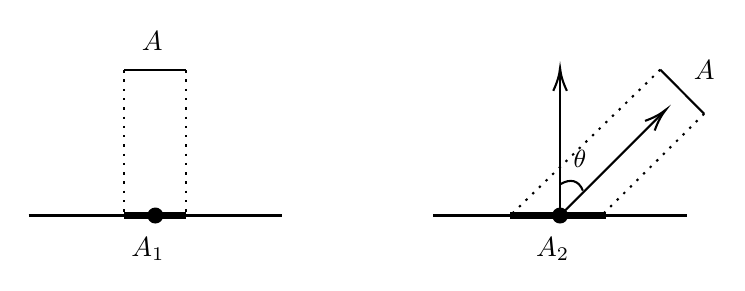
\begin{tikzpicture}[x=0.75pt,y=0.75pt,yscale=-1,xscale=1]
    %uncomment if require: \path (0,300); %set diagram left start at 0, and has height of 300
    
    %Straight Lines [id:da170514078900192] 
    \draw    (54,230) -- (176,230) ;
    \draw [shift={(115,230)}, rotate = 0] [color={rgb, 255:red, 0; green, 0; blue, 0 }  ][fill={rgb, 255:red, 0; green, 0; blue, 0 }  ][line width=0.75]      (0, 0) circle [x radius= 3.35, y radius= 3.35]   ;
    %Straight Lines [id:da016015541896946983] 
    \draw    (100,160) -- (130,160) ;
    %Straight Lines [id:da2875279917672757] 
    \draw  [dash pattern={on 0.84pt off 2.51pt}]  (100,160) -- (100,230) ;
    %Straight Lines [id:da4948721440011248] 
    \draw  [dash pattern={on 0.84pt off 2.51pt}]  (130,160) -- (130,230) ;
    %Straight Lines [id:da6791345652096885] 
    \draw [line width=2.25]    (100,230) -- (130,230) ;
    %Straight Lines [id:da17937256958328818] 
    \draw    (249,230) -- (371,230) ;
    \draw [shift={(310,230)}, rotate = 0] [color={rgb, 255:red, 0; green, 0; blue, 0 }  ][fill={rgb, 255:red, 0; green, 0; blue, 0 }  ][line width=0.75]      (0, 0) circle [x radius= 3.35, y radius= 3.35]   ;
    %Straight Lines [id:da5726229973180355] 
    \draw    (358.31,159.71) -- (379.42,181.02) ;
    %Straight Lines [id:da01972159484297009] 
    \draw  [dash pattern={on 0.84pt off 2.51pt}]  (358.31,159.71) -- (286,230) ;
    %Straight Lines [id:da8044979993297667] 
    \draw  [dash pattern={on 0.84pt off 2.51pt}]  (379.42,181.02) -- (329.69,230.29) ;
    %Straight Lines [id:da7389754977606782] 
    \draw [line width=2.25]    (286,230) -- (332,230) ;
    %Straight Lines [id:da7593939440598445] 
    \draw    (310,230) -- (310,161) ;
    \draw [shift={(310,159)}, rotate = 450] [color={rgb, 255:red, 0; green, 0; blue, 0 }  ][line width=0.75]    (10.93,-3.29) .. controls (6.95,-1.4) and (3.31,-0.3) .. (0,0) .. controls (3.31,0.3) and (6.95,1.4) .. (10.93,3.29)   ;
    %Straight Lines [id:da5048921054355329] 
    \draw    (310,230) -- (359.59,180.41) ;
    \draw [shift={(361,179)}, rotate = 495] [color={rgb, 255:red, 0; green, 0; blue, 0 }  ][line width=0.75]    (10.93,-3.29) .. controls (6.95,-1.4) and (3.31,-0.3) .. (0,0) .. controls (3.31,0.3) and (6.95,1.4) .. (10.93,3.29)   ;
    %Curve Lines [id:da665946044320908] 
    \draw    (310,215) .. controls (315,212) and (319,213) .. (321,218) ;
    
    % Text Node
    \draw (107,140) node [anchor=north west][inner sep=0.75pt]   [align=left] {$\displaystyle A$};
    % Text Node
    \draw (102,239) node [anchor=north west][inner sep=0.75pt]   [align=left] {$\displaystyle A_{1}$};
    % Text Node
    \draw (373,154) node [anchor=north west][inner sep=0.75pt]   [align=left] {$\displaystyle A$};
    % Text Node
    \draw (297,239) node [anchor=north west][inner sep=0.75pt]   [align=left] {$\displaystyle A_{2}$};
    % Text Node
    \draw (315,197) node [anchor=north west][inner sep=0.75pt]  [font=\small] [align=left] {$\displaystyle \theta $};
    
    
    \end{tikzpicture}
    

\caption{Example: on the right, the differential area $A_2$ illuminated by the ray is larger, because the ray is not perpendicular to the plane.}    
\end{figure}


\subsection{The BRDF}

In order to accurately model the incoming and outgoing radiances at each point, it is essential to take into account the fact that surfaces can reflect incoming light. That is, for any direction $\omega_i$, the incoming radiance $L_i(p,\omega_i)$ can contribute to the outgoing radiance $L_o(p,\omega_o)$ of another direction $\omega_o$. For each surface point, this relationship is captured by the bi-directional reflectance distribution function (BRDF), written as $f_r(p,\omega_o,\omega_i)$. Formally, the BRDF is defined as 
\begin{align}
    f_r(p,\omega_o,\omega_i) = \frac{dL_o(p,\omega_o)}{dE(p,\omega_i)}
    \label{BRDF def 1}
\end{align}
where $dE(p,\omega_i)$ represents the differential incoming irradiance in the direction $\omega_i$.

Using equation \ref{radiance integral}, it can be derived that 
\begin{align}
    dE(p,\omega_i) = L_i(p,\omega_i)\cos\theta_id\omega_i
\end{align}
which allows equation \ref{BRDF def 1} to be re-written as
\begin{align}
    f_r(p,\omega_o,\omega_i) = \frac{dL_o(p,\omega_o)}{L_i(p,\omega_i)\cos\theta_id\omega_i}
\end{align}
From this, it's straightforward to show that
\begin{align}
    L_o(p,\omega_o) = \int_\Omega L_i(p,\omega_i)f_r(p,\omega_o,\omega_i)\cos\theta_id\omega_i + C
    \label{reflection plus C}
\end{align}
for some $C$.

Equation \ref{reflection plus C} shows that, given the incident radiances and the BRDF, the portion of outgoing radiances caused by reflections can be computed. As a result, the BRDF of a surface completely decides how the surface reflects light, which is a crucial factor of its appearances when viewed by a camera. Different materials in the real world have drastically different BRDFs, and it's vital for a physically based renderer to accurately implement these functions, if photorealistic images are to be rendered. A family of BRDFs known for their physical accuracy are the Microfacet BRDFs, which are well implemented by this project. Unfortunately, due to the complexity of these models, details of these BRDFs could not be described here. 
\begin{figure}[H]
    \centering
    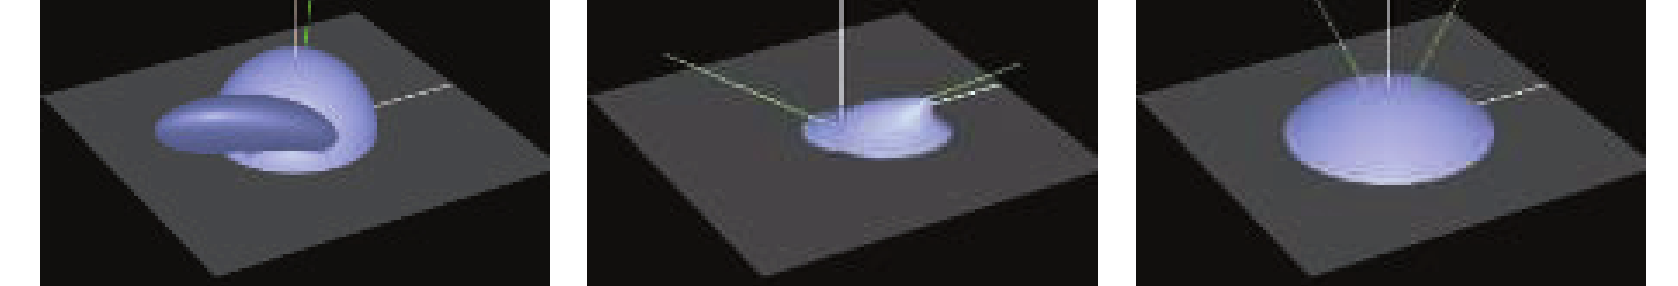
\includegraphics[scale = 0.6]{brdfs}
    \caption{Shapes of example BRDFs. Image credit\cite{akenine2019real}}
\end{figure}

In order to fully model $L_o(p,\omega_o)$, it remains to describe the term $C$ in equation \ref{reflection plus C}. Surfaces in the real world sends outgoing radiances for two reasons only: they might emit light actively, and they reflect incoming light. Equation \ref{reflection plus C} already includes the reflected radiances, and thus it only remains to include actively emitted light. Writing $L_e(p,\omega_o)$ for the actively emitted radiance from $p$ towards the direction $\omega_o$, the following equation completely describes $L_o$:
\begin{align}
    L_o(p,\omega_o) = L_e(p,\omega_o) + \int_\Omega L_i(p,\omega_i)f_r(p,\omega_o,\omega_i)\cos\theta_id\omega_i
    \label{rendering equation}
\end{align}
which is the famous rendering equation, originally proposed by Kaijiya\cite{rendering_equation}. 


Under the assumption that radiance is constant along each ray, the incoming radiance $L_i(p,\omega_i)$ can be equated with the outgoing radiance from another point, $q$, as illustrated below.
\begin{figure}[H]
    \centering
    


\tikzset{every picture/.style={line width=0.75pt}} %set default line width to 0.75pt        

\begin{tikzpicture}[x=0.75pt,y=0.75pt,yscale=-1,xscale=1]
%uncomment if require: \path (0,300); %set diagram left start at 0, and has height of 300

%Straight Lines [id:da05220876887007719] 
\draw    (30,260) -- (211,260) ;
\draw [shift={(120.5,260)}, rotate = 0] [color={rgb, 255:red, 0; green, 0; blue, 0 }  ][fill={rgb, 255:red, 0; green, 0; blue, 0 }  ][line width=0.75]      (0, 0) circle [x radius= 3.35, y radius= 3.35]   ;
%Straight Lines [id:da8868681333199677] 
\draw    (150,230.5) -- (121.91,258.59) ;
\draw [shift={(120.5,260)}, rotate = 315] [color={rgb, 255:red, 0; green, 0; blue, 0 }  ][line width=0.75]    (10.93,-3.29) .. controls (6.95,-1.4) and (3.31,-0.3) .. (0,0) .. controls (3.31,0.3) and (6.95,1.4) .. (10.93,3.29)   ;
%Image [id:dp7926495246340768] 
\draw (232,169) node  {
\includegraphics[width=27pt,height=30pt]{lightbulb.png}};
%Straight Lines [id:da34057240843922076] 
\draw  [dash pattern={on 0.84pt off 2.51pt}]  (150,230.5) -- (180,200) ;
%Straight Lines [id:da8846910740201797] 
\draw    (210,170) -- (181.41,198.59) ;
\draw [shift={(180,200)}, rotate = 315] [color={rgb, 255:red, 0; green, 0; blue, 0 }  ][line width=0.75]    (10.93,-3.29) .. controls (6.95,-1.4) and (3.31,-0.3) .. (0,0) .. controls (3.31,0.3) and (6.95,1.4) .. (10.93,3.29)   ;

% Text Node
\draw (141,272) node [anchor=north west][inner sep=0.75pt]   [align=left] {$\displaystyle p$};
% Text Node
\draw (255,155) node [anchor=north west][inner sep=0.75pt]   [align=left] {$\displaystyle q$};
% Text Node
\draw (123,163) node [anchor=north west][inner sep=0.75pt]   [align=left] {$\displaystyle L_{o}( q,-\omega _{i})$};
% Text Node
\draw (64,224) node [anchor=north west][inner sep=0.75pt]   [align=left] {$\displaystyle L_{i}( p,\omega _{i})$};


\end{tikzpicture}

\end{figure} 
Thus, defining the ray-tracing function $t(p,\omega_i)$ as a function that computes the first surface point $q$ intersected by a ray from $p$ in the direction $\omega_i$, the rendering equation is re-written in a new form:
\begin{align}
    L_o(p,\omega_o) = L_e(p,\omega_o) + \int_\Omega L_o(t(p,\omega_i),-\omega_i)f_r(p,\omega_o,\omega_i)\cos\theta_id\omega_i
    \label{rendering equation with cast}
\end{align}
Finding solutions to this equation is the ultimate goal of rendering, because the job of any renderer is to compute the amount of radiance received by a hypothetical camera placed in the scene. In other words, for each point $p$ that is visible from the camera, the rendering algorithm must compute $L_o(p,\omega_o)$, where $\omega_o$ points from $p$ towards the camera. The following section will begin the discussion of how this equation is solved in practice.

\section{Monte Carlo Integration}

Equation \ref{rendering equation with cast} cannot be solved analytically for all but the simplest scenes. Thus, rendering software solve the equation numerically using the method of Monte Carlo integration. Given an integral
\begin{align*}
    I = \int_\Omega f(x) dx,
\end{align*}
the Monte Carlo estimator randomly samples $N$ points $x_1,...,x_n\in \Omega$ according to some distribution $D$, and computes
\begin{align}
    I_N = \frac{1}{N}\sum_{i=1}^{N} \frac{f(x_i)}{p(x_i)}
    \label{monte carlo estimator}
\end{align}
where $p(x_i)$ is the probability density of sampling $x_i$ according to $D$. It can be proved that this indicator is both unbiased $(E[I_N]=I)$ and consistent $(\lim_{N\to\infty}I_N = I)$. When applied to the rendering equation, the support $\Omega$ is the sphere or hemisphere of directions, and the function $f$ is computed by recursively estimating $L_o$, and then multiplying by the BRDF and the cosine of the direction.

\subsection{Importance Sampling}

In rendering, the variance $\Var[I_N]$ of the Monte Carlo estimator manifest in the form of random noise in the resulting image. Thus, variance reduction techniques are vital for rendering high-quantity images efficiently. One of the most important such techniques is importance sampling.

In the monte carlo estimator, the distribution $D$ used can be an arbitrary distribution. However, different distributions can lead to dramatically different variances. Importance sampling uses the fact that, informally, the variance $\Var[I_N]$ is reduced as the shape of the PDF $p(x)$ becomes similar to the shape of the integrand $f(x)$. As an example, consider when the PDF is 
$$ 
p(x)=\frac{f(x)}{\int_\Omega f(x') dx'}.
$$ 
In this case, $p$ is always proportional to $f$, and the variance of the estimator is
\begin{align*}
\Var[I_N]
&= \frac{1}{N}\Var_{x\sim D}\left[\frac{f(x)}{p(x)}\right]\\
&= \frac{1}{N}\Var_{x\sim D}\left[\int_\Omega f(x') dx'\right]\\
&=0
\end{align*}
It is of course infeasible to obtain a perfectly proportional PDF, because doing so requires computing the value of $\int_\Omega f(x') dx'$, which is the value to be estimated in the first place. However, even if $p$ is similar in shape to $f$, variance can still be reduced.

\subsection{Multiple Importance Sampling}
\label{subsection MIS}
When solving the rendering equation, the integrand is the product of two factors: the incoming radiance $L_o(t(p,\omega_i),-\omega_i)$, and the reflectance $f_r(p,\omega_o,\omega_i)\cos\theta_i$. More generally, the renderer is solving an integration of the form
$$
I = \int_\Omega f(x)g(x)dx
$$

In this case, if the renderer were to perform importance sampling to estimate this integral according to distributions based on either $f$ or $g$, one of these two will often perform poorly\cite{pharr2016physically}. This is exactly the issue addressed by the technique of multiple importance sampling, or MIS.

The basic idea of MIS is that, when estimating an integral, samples should be drawn from multiple distributions, chosen in the hope that at least one will match the shape of the integrand well. MIS provides a method of weighting the samples from each distribution that eliminates large variance spikes due to mismatches between the integrand and the sampling density. More precisely, given a PDF $p_f$ that is a good match for $f$, and $p_g$ that is a good match for $g$, MIS proposes to $N$ samples $x_1,...,x_N$ from $p_f$, and $y_1,...,y_N$ from $p_g$, and apply the alternative Monte Carlo estimator:
\begin{align}
    I_N = \frac{1}{N} \sum_{i=1}^{N} \frac{f(x_i)g(x_i)w_f(x_i)}{p_f(x_i)} + \frac{f(y_i)g(y_i)w_g(y_i)}{p_g(y_i)}
    \label{MIS}
\end{align}
where the weights $w_f$ and $w_g$ are defined by
\begin{align*}
    w_s(x) = \frac{p_f(x)^2}{p_f(x)^2+p_g(x)^2}
\end{align*}
A full recount of why this weighting scheme reduces variance can be found in \cite{pharr2016physically}. 

In order to apply MIS to solving the rendering equation, the renderer need to sample from a PDF $p_{rad}$ which matches to the incoming radiance $L_o(t(p,\omega_i),-\omega_i)$, and another PDF $p_{ref}$ which matches the reflection term $f_r(p,\omega_o,\omega_i)\cos\theta_i$. In the path-tracing algorithm implemented by this project, $p_{rad}$ is a distribution which only samples $\omega_i$ that points to a light source, which is often much brighter than surfaces that indirectly reflects light. For $p_{ref}$, which corresponds to surface reflection and is thus material dependent, the project implemented specific sampling routings for each individual material, thereby maximizing the similarity between the PDF and the BRDF of the materials. 


\section{The Path Space Formulation}
The rendering equation as written in equation \ref{rendering equation with cast} is inconvenient for deriving algorithms, because the relationship between geometries in the scene is implicit in the ray-tracing function $t(p,\omega_i)$. This section rewrites the equation into a from that makes this relationship more explicit.

Firstly, equation \ref{rendering equation with cast} is to be transformed from an integral over directions into an integral over area. More precisely, the variable of integration $\omega_i$, which represents an incoming direction, is to be replaced by a point $p_{src}$, which represents the source of the incoming ray. To achieve this change of variable, for any two points $p,p'$ that are mutually visible, define 
\begin{align*}
    L_o(p'\to p) = L_o(p',\omega)\\
    L_e(p'\to p) = L_e(p',\omega)
\end{align*}
where $\omega = \frac{p-p'}{|p-p'|}$. Similarly, for three points $p,p',p''$, such that $p$ is visible from $p'$ and $p'$ is visible from $p''$, the BRDF at $p'$ is written as
\begin{align*}
    f_r(p''\to p'\to p) = f_r(p',\omega_o,\omega_i)
\end{align*} 
where $\omega_i = \frac{p''-p'}{|p''-p'|}$ and $\omega_o = \frac{p-p'}{|p-p'|}$.

Note that, since not all points $p_{src}$ is visible from $p$, the integrand needs to include a visibility term $V(p,p_{src})$, which takes the value 1 if $p_{src}$ is visible from $p$, and 0 otherwise. Furthermore, the change of variable also incurs a Jacobian term, which is $\frac{\cos\theta'}{|p-p_{src}|^2}$, with $\theta'$ being the angle between the incoming ray and the surface normal at $p_{src}$. Use these terms, equation \ref{rendering equation with cast} is rewritten so that for a ray from a point $p$ to the destination $p_{dest}$, the radiance is computed by
\begin{align*}
    L_o(p\to p_{dest}) =~ &L_e(p\to p_{dest}) \\
    &+ \int_A f_r(p_{src}\to p\to p_{dest}) L_o(p_{src}\to p)  V(p,p_{src}) \frac{cos\theta\cos\theta'}{|p-p_{src}|^2} d p_{src}
\end{align*} 
where $A$ is the domain of all surface points in the scene. To simplify notation, write the term $G(p,p_{src})$ as $V(p,p_{src}) \frac{cos\theta\cos\theta'}{|p-p_{src}|^2}$, the equation becomes
\begin{align*}
    L_o(p\to p_{dest}) =~ &L_e(p\to p_{dest}) \\
    &+ \int_A f_r(p_{src}\to p\to p_{dest}) L_o(p_{src}\to p)  G(p,p_{src})  d p_{src}
\end{align*} 

The equation above is referred to as the surface form light transport equation, and it can be interpreted as a recursive definition for $L_o$. Naturally, one can expand this recursive definition, and obtain an infinite sum:
\begin{align*}
    L_o(p_1\to p_0) =
    &L_e(p_1\to p_0)\\
    &+ \int_A L_e(p_2\to p_1)f_r(p_2\to p_1\to p_0)G(p_2,p_1) dp_2\\
    &+ \int_A \int_A L_e(p_3\to p_2)f_r(p_3\to p_2\to p_1) G(p_3,p_2)f(p_2\to p_1\to p_0)G(p_2,p_1) ~ dp_3dp_2\\
    &+~...
\end{align*}
Here, each term represents the radiance contributed by paths of increasing length. For example, the first term in the sum represents the radiance directly emitted at $p_1$; the second term represents the radiance emitted at some point $p_2$ and reflected at $p_1$; the third term represents the radiance emitted at $p_3$ and reflected at $p_2$ and then again at $p_1$, and so on. For a path with $n$ reflection points, the source emission is $L_e(p_{n+1}\to p_{n})$, and it is weighted by a throughput term $T_n$, which is the product of the $f_r$ and $G$ at each reflection point:
\begin{align*}
    T_n = \prod_{i=1}^{n} f_r(p_{n+1}\to p_n\to p_{n-1})G(p_{n+1},p_n)
\end{align*}
which allows the previous equation to be written as
\begin{align*}
    L_o(p_1\to p_0) = \sum_{n=0}^{\infty} \underbrace{\int_A \int_A...\int_A}_{n} L_e(p_{n+1}\to p_{n})T_n dp_{n}dp_{n-1}...dp_1
\end{align*}

Notice that, the throughput term $T_n$ computes the portion of radiance that remains after $n$ reflections, which tends to decrease exponentially as $n$ increases. For this reason, it is natural to only consider the first few terms of this infinite sum. More precisely, given a maximum amount of reflections $MaxDepth$, the radiance $L_o(p_1\to p_0)$ can be estimated by 
\begin{align}
    L_o(p_1\to p_0) = \sum_{n=0}^{MaxDepth} \underbrace{\int_A \int_A...\int_A}_{n} L_e(p_{n+1}\to p_{n})T_n dp_{n}dp_{n-1}...dp_1
    \label{rendering equation path tracing}
\end{align}

If a Monte Carlo estimator is used to approximate the value for each integral, the above formula becomes a recipe for a practical algorithm for computing radiances. This leads to the famous algorithm known as path-tracing, which is described in the next section.

\section{The Path-Tracing Algorithm}
The input of the path-tracing algorithm is a scene, defined by its geometries and materials, together with a camera, defined by its position, orientation, image resolution, and field of view (FOV) angle. Additionally, the algorithm is also parameterized by an integer $spp$, which stands for samples per pixel.

For each pixel on the image, the path-tracing algorithm samples $spp$ random points on the pixel. For each of these random points, the algorithm generates $1+MaxDepth*2$ paths of increasing length, and accumulates the radiance carried by these paths. Finally, the radiances for all sample points in each pixel are combined by a Monte Carlo estimator, which decides the final value of the pixel.

The path tracing algorithm generates paths incrementally, where previous reflection points are reused. More precisely, after generating $n$ reflection points $p_1,...,p_n$ , whose throughput is $T_n$, the algorithm does the following:


\begin{algorithm}[H]
    \label{Path construction}
    \SetKwProg{Fn}{Function}{:}{end}
    
    Samples a point $p_{light}$ from a light source.\;

    Test whether the ray $p_{light}\to p_n$ is occluded by some geometry. If not, then this generates a path of $n$ reflections, whose radiance is to be accumulated\;

    Sample a direction $\omega_i$ from a distribution that matches the BRDF at $p_n$\;

    Trace the ray with origin $p_n$ and direction $\omega_i$. Let the intersection with the scene be $p_{n+1}$\;

    If $p_{n+1}$ is on a light source, then again this leads is a path of $n$ reflections, whose radiance is accumulated\;


    Let $p_{n+1}$ be the next reflection point\;

    Let $T_{n+1}$ be $T_n  f_r(p_{n+1}\to p_n\to p_{n-1})G(p_{n+1},p_n)$\;

    \caption{Incremental Path Construction}
\end{algorithm}

~

Notice that, step 2 and 5 are two different ways a light emitter can illuminate the pont $p_n$, and these two different paths exactly correspond to Multiple Importance Sampling, described in subsection \ref{subsection MIS}. Thus, when accumulating their radiances, the MIS weight should be applied.

To summarize, the path-tracing algorithm works as follows:


\begin{algorithm}[H]
    \label{Path Tracing}
    \SetKwProg{Fn}{Function}{:}{end}
    \ForEach{\upshape pixel in the image}{
        \For{\upshape $i$ from 1 to $spp$}{
            Let $p_0$ be the location of the camera\;
            Randomly select a location inside the pixel, and generate a ray $r$ corresponding to this location\;
            Compute the first intersection point $p_1$ between $r$ and the scene\;
            Accumulate $L_e(p_1\to p_0)$\;
            \For{\upshape $n$ from $1$ to $MaxDepth$}{
                Incrementally construct two further paths, using algorithm \ref{Path construction}\;
                Accumulate the radiances from the newly generated paths, weighted by MIS\;
            }
        }
        Combine radiances computed by each sample to obtain final color of pixel\;
    }
    \caption{Path Tracing}
\end{algorithm}

This algorithm is now the corner stone of photorealistic rendering. The remainder of this report will discuss the problem of efficiently implementing it on GPUs, and a variant of this algorithm where Reinforcement Learning is used to make smarter choices during importance sampling.